\section{Leibniz, Gauss-Bonnet, Poincaré-Hopf}

\subsection{The Leibniz (product) rule}

The intuition that motivates everything in this note is that derivatives and connections are visible in type theory through the action on paths, because a path is a finite version of an infinitesimal tangent vector. And if we think we have some new understanding of differentiation, then we should be able to see the Leibniz rule.

The Leibniz rule, or product rule, for differentiation states that if \( f, g:M\to \rr \) are two smooth functions to the real numbers then \( d(fg) = fdg + gdf \). Here \( fg \) is the function formed by taking the pointwise product of \( f \) and \( g \). This is an interaction between multiplication in \( \rr \) and the action on vectors of smooth functions (the 1-forms \( df \) and \( dg \)). 

To examine this situation in HoTT we need type-theoretic functions \( f, g:M\to B \) from some type \( M \) to a central H-space \( B \). Let \( \mu:B\to B\to B \) be the H-space multiplication. How does \( \mu \) act on paths? Suppose we have \( a, a', b, b':B \) and \( p:a=_B a', q:b=_B b' \). Then we also have homotopies \( \mu(p, -):\mu(a, -)=_{B\to B}\mu(a', -) \) and \( \mu(-,q):\mu(-,b)=_{B\to B}\mu(-,b'). \) Since \( \mu(a, -):B=B \) is an (unpointed) equivalence of \( B \), and similarly for \( \mu(b, -) \) and so on, this data assembles into the following diagram of higher groupoid morphisms:

\begin{center}
% https://q.uiver.app/#q=WzAsMyxbMiwwLCJCIl0sWzAsMCwiQiJdLFs0LDAsIkIiXSxbMSwwLCJcXG11KGEsLSkiLDAseyJjdXJ2ZSI6LTN9XSxbMSwwLCJcXG11KGEnLC0pIiwyLHsiY3VydmUiOjN9XSxbMCwyLCJcXG11KC0sYikiLDAseyJjdXJ2ZSI6LTN9XSxbMCwyLCJcXG11KC0sYicpIiwyLHsiY3VydmUiOjN9XSxbMyw0LCJcXG11KHAsLSkiLDIseyJzaG9ydGVuIjp7InNvdXJjZSI6MjAsInRhcmdldCI6MjB9fV0sWzUsNiwiXFxtdSgtLHEpIiwyLHsic2hvcnRlbiI6eyJzb3VyY2UiOjIwLCJ0YXJnZXQiOjIwfX1dXQ==
\begin{tikzcd}
  B && B && B
  \arrow[""{name=0, anchor=center, inner sep=0}, "{\mu(a,-)}", curve={height=-18pt}, from=1-1, to=1-3]
  \arrow[""{name=1, anchor=center, inner sep=0}, "{\mu(a',-)}"', curve={height=18pt}, from=1-1, to=1-3]
  \arrow[""{name=2, anchor=center, inner sep=0}, "{\mu(-,b)}", curve={height=-18pt}, from=1-3, to=1-5]
  \arrow[""{name=3, anchor=center, inner sep=0}, "{\mu(-,b')}"', curve={height=18pt}, from=1-3, to=1-5]
  \arrow["{\mu(p,-)}"', shorten <=5pt, shorten >=5pt, Rightarrow, from=0, to=1]
  \arrow["{\mu(-,q)}"', shorten <=5pt, shorten >=5pt, Rightarrow, from=2, to=3]
\end{tikzcd}
\end{center}

And so the two homotopies can be horizontally composed to give a path \[ \mu(p,-)\star\mu(-,q): \mu(a, b)=\mu(a',b'). \] Horizontal composition is given by \[\mu(p,-)\star\mu(-,q)\defeq(\mu(p,-)\cdot_r \mu(-,b))\cdot(\mu(a', -)\cdot_l\mu(-, q))\] where \[ \mu(p,-)\cdot_r\mu(-,b):\mu(a,b)=\mu(a',b) \] and \[ \mu(a',-)\cdot_l\mu(-,q):\mu(a',b)=\mu(a',b') \] are defined by path induction.  See the HoTT book Theorem 2.1.6 on the Eckmann-Hilton argument\cite{hottbook}.

We can recognize the process of using whiskering to form horizontal composition in the Leibniz rule. 

Quick aside: moving from infinitesimal calculus to finite groupoid algebra actually involves two changes. The first is the change from vectors to paths, forms to functions and so on. But it's also the case that tangent vectors have just the one basepoint, whereas paths have two endpoints. You can see this play out in this example, where \( a \) and \( a' \) were distinct points (and \( b \) and \( b' \)).

The horizontal composition we build lives entirely in \( B \) and we didn't make use of \( M \) yet. The Leibniz rule will be a pointwise version of what's going on in \( B \). Denote by \( \mu\circ(f,g):M\to B \) the map which sends \( x\mapsto \mu(f(x),g(x)) \).

\begin{mylemma}
Given \( f, g:M\to B \) and \( p:x=_M y \) then 
\begin{align*}
 \ap(\mu\circ(f,g))(p)&=\mu(f(p),-)\star\mu(-,g(p))\\
 &=\left[\mu(f(p),-)\cdot_r \mu(-,g(x))\right]\cdot \left[\mu(f(y),-)\cdot_l\mu(-,g(p))\right]\\
 &:\mu(f(x),g(x))=\mu(f(y),g(y))
\end{align*}
\end{mylemma}

\subsection{The total curvature}

\begin{mydef}
Let \( F(M) \) denote the groupoid of faces of \( M \) generated by the faces in its constructor. Let \( V:\pit{f:F(M)}f \) be a selected vertex of every face, and let \( \partial:\pit{f:F(M)}Vf=_M Vf \) be the clockwise boundary path around a face. Let \( v \) be the basepoint of \( M \). Then in particular we have \( M:F(M) \) the concatenation of all faces (i.e. \( M \) itself), and we have \( \partial(M):v=_M v \) which is the concatenation of all boundaries.
\end{mydef}

Observe that each generating edge of \( M \) is visited once in each direction in the concatenation \( \partial(M) \). 

The bundle map \( T \) can be examined on each face. On a face \( f \) bounding a loop \( \ell:v=_M v \) the map \( T:M\to\EMzo \) assigns a homotopy \( T(f):\refl_v=T(\ell) \), where \( T(\ell) \) is an automorphism of \( T(v) \). On the composition of all faces we have \( T(M):T(v)=T(v) \), the \defemph{total curvature}.

It is crucial that \( T(M) \) can be nontrivial (i.e. not \( \refl_v \)) even though it's computed by transporting across every edge in \( \partial(M) \) once in each direction!

\subsection{The total index}

See Figure~\ref{fig:torus_morse} where the outlined hexagons are the composition of the six triangular faces around a zero.

If \( X \) is a vector field with isolated zeros on \( Z \), then \( M_Z \) is a convenient replacement for \( M \) because \( X \) is a partial function defined on all of \( M_Z \) except for a collection of faces, each of which bounds one of the zeros of \( Z \).

\begin{mynote}
If the combinatorial manifold was imported into type theory via some process of sampling or other, perhpaps more theoretical, construction then we should allow for zeros to occur on verticies, edges, or faces. We can reduce the case of a zero on a vertex or edge to that of a face with the replacement method just described. The original combinatorial neighborhood structure continues to live in the fibers of \( T \), it's only the base manifold that has been replaced.
\end{mynote}

\begin{mydef}
Given a face \( f:F(M\setminus Z) \), define \defemph{the index of \( X \) on \( f \)} to be the winding number (also called the degree) of \( X(\partial f) \). The \defemph{total index} of \( X \) on \( M\setminus Z \) is the index of \( X \) on \( \partial(M\setminus Z) \).
\end{mydef}

The index computation skips some faces of \( M \) and can most definitely be nonzero.

\subsection{Equality of total index and total curvature}

Here we closely follow the classical proof of Hopf\cite{hopf}, presented in detail in Needham\cite{needham}.

\begin{mythm}
The total curvature's winding number is equal to the total index of \( X \).
\end{mythm}
The fact that the index was already an integer, whereas the curvature is a path accounts for the factor of \( 2\pi \) in some classical statement of this theorem (e.g. \cite{needham} section 26.3).
\begin{proof}
Let \( C \) be a fixed pointed polygon (e.g. \( C_4 \) or \( C_6 \) which we met earlier). We can consider \( X \) to map each vertex of \( M_Z \) to \( C \). On each face of \( M_Z \) (no faces are omitted) we traverse the boundary, which is in the domain of both \( T \) and of \( X \). So we avoid the complication that \( X \) is not defined on some of the faces by remaining on the 1-skeleton. For a given edge \( e_{12}:v_1=_{M_Z} v_2 \) the function \( \tr_{e_{12}}X(v_1)=X(v_2) \) is a path in \( C \). We will traverse every edge twice, once in each direction, which will cancel to give \( \refl_v \). In particular the boundaries around the zeros of \( X \) are themselves traversed twice in opposite directions, canceling the total index.
\end{proof}

\begin{mycor}
The total index of a vector field with isolated zeros is independent of the vector field.
\end{mycor}

\begin{mycor}
The total curvature is an integer.
\end{mycor}

The last step is to link this value to the Euler characteristic.

\subsection{Identification with Euler characteristic}

Combinatorial manifolds are intuitive objects that connect directly to the classical definition of Euler characteristic. We can argue using Morse theory, the study of smooth real-valued functions on smooth manifolds and their singularities. Classically the gradient of a Morse function is a vector field that can be used to decompose the manifold into its \emph{handlebody decomposition}. This would be an excellent story to pursue in future work.

Imagine a combinatorial manifold of a genus g oriented surface standing upright with the holes forming a vertical sequence. Now install a vector field that points downward whenever possible. This vector field will have a zero at the top and bottom, and one at the top and bottom of each hole. The top and bottom will be index 1, and ones around the holes will be index -1. We include some sketches in the case of a torus. This illustrates how we obtain the formula for genus \( g \): \( \chi(M)=2-2g \).

\begin{figure}[htbp]
\centering
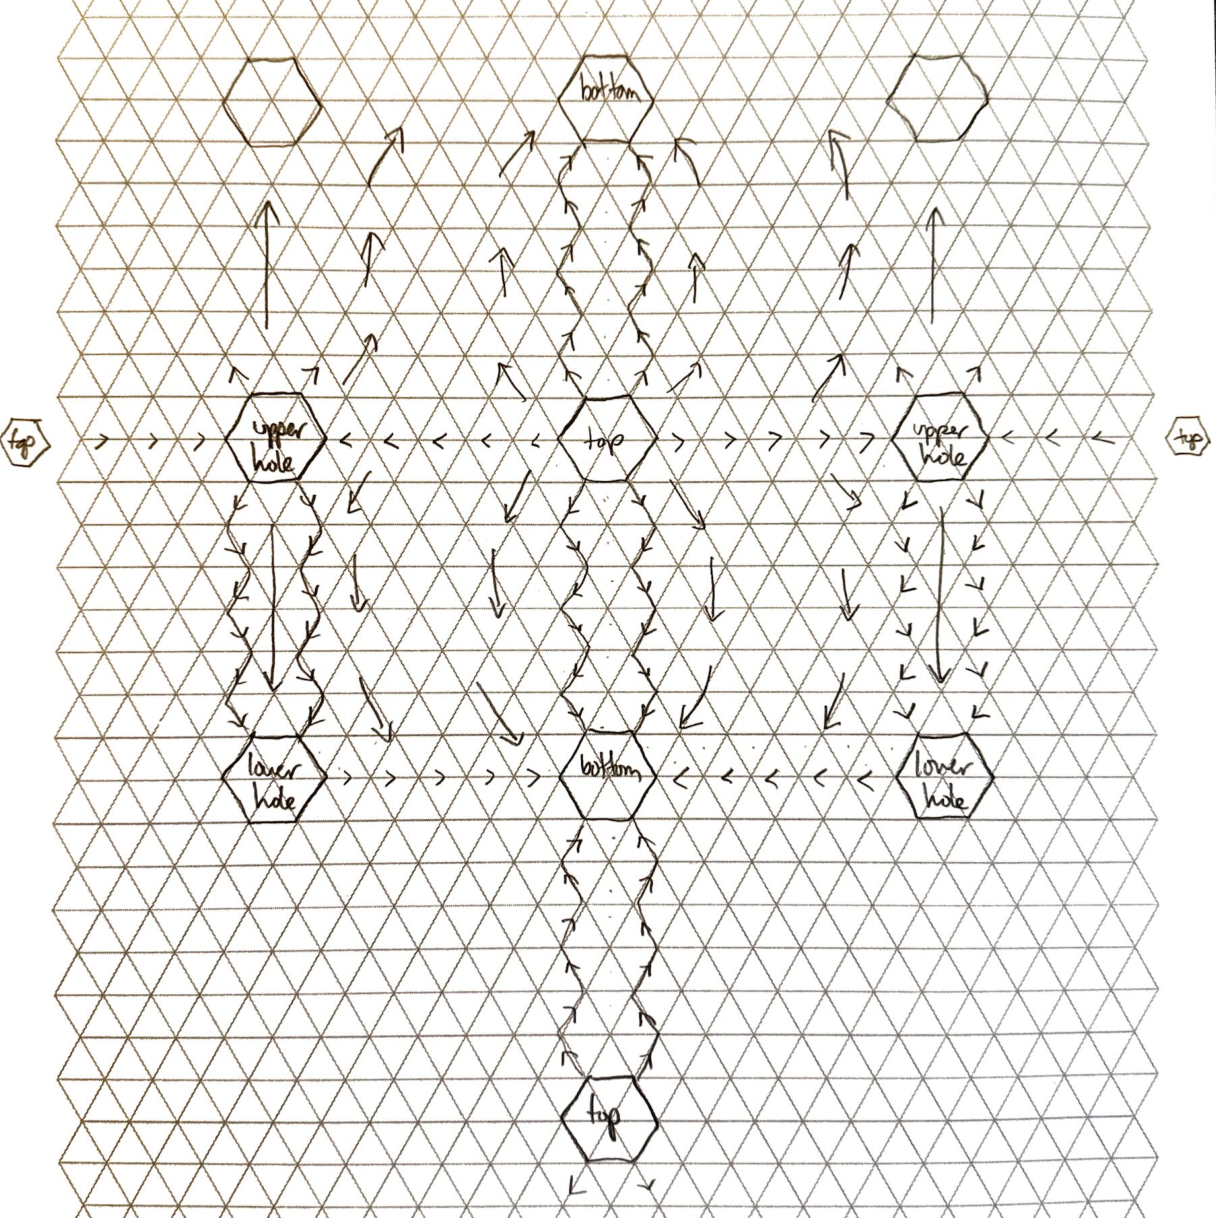
\includegraphics[width=400pt]{torus_morse_grad.pdf}
\caption{A sketch of downward flow on the torus.}
\label{fig:torus_morse}
\end{figure}

\begin{figure}[htbp]
\centering
% https://q.uiver.app/#q=WzAsOCxbMCwwLCJcXGJ1bGxldCJdLFswLDEsIlxcYnVsbGV0Il0sWzAsMiwiXFxidWxsZXQiXSxbMCwzLCJcXGJ1bGxldCJdLFsxLDAsIlxcbWF0aHJte3RvcH0iXSxbMSwxLCJcXG1hdGhybXt1cHBlclxcIGhvbGV9Il0sWzEsMiwiXFxtYXRocm17bG93ZXJcXCBob2xlfSJdLFsxLDMsIlxcbWF0aHJte2JvdHRvbX0iXSxbMCwxLCIiLDIseyJjdXJ2ZSI6LTEsInN0eWxlIjp7ImJvZHkiOnsibmFtZSI6ImRhc2hlZCJ9fX1dLFswLDEsIiIsMCx7ImN1cnZlIjoxLCJzdHlsZSI6eyJib2R5Ijp7Im5hbWUiOiJkYXNoZWQifX19XSxbMiwzLCIiLDAseyJjdXJ2ZSI6LTEsInN0eWxlIjp7ImJvZHkiOnsibmFtZSI6ImRhc2hlZCJ9fX1dLFsyLDMsIiIsMix7ImN1cnZlIjoxLCJzdHlsZSI6eyJib2R5Ijp7Im5hbWUiOiJkYXNoZWQifX19XSxbMCwzLCIiLDEseyJjdXJ2ZSI6LTV9XSxbMCwzLCIiLDEseyJjdXJ2ZSI6NX1dLFsxLDIsIiIsMSx7ImN1cnZlIjoyfV0sWzEsMiwiIiwxLHsiY3VydmUiOi0yfV1d
\begin{tikzcd}[cramped]
  \bullet & {\mathrm{top}} \\
  \bullet & {\mathrm{upper\ hole}} \\
  \bullet & {\mathrm{lower\ hole}} \\
  \bullet & {\mathrm{bottom}}
  \arrow[curve={height=-6pt}, dashed, from=1-1, to=2-1]
  \arrow[curve={height=6pt}, dashed, from=1-1, to=2-1]
  \arrow[curve={height=-30pt}, from=1-1, to=4-1]
  \arrow[curve={height=30pt}, from=1-1, to=4-1]
  \arrow[curve={height=12pt}, from=2-1, to=3-1]
  \arrow[curve={height=-12pt}, from=2-1, to=3-1]
  \arrow[curve={height=-6pt}, dashed, from=3-1, to=4-1]
  \arrow[curve={height=6pt}, dashed, from=3-1, to=4-1]
\end{tikzcd}
\caption{Schematic of the zeros of the downward flow of a torus.}
\label{fig:torus_morse_skel}
\end{figure}
